\PassOptionsToPackage{unicode=true}{hyperref} % options for packages loaded elsewhere
\PassOptionsToPackage{hyphens}{url}
%
\documentclass[pdf]{apa6}
\usepackage{lmodern}
\usepackage{amssymb,amsmath}
\usepackage{ifxetex,ifluatex}
\usepackage{fixltx2e} % provides \textsubscript
\ifnum 0\ifxetex 1\fi\ifluatex 1\fi=0 % if pdftex
  \usepackage[T1]{fontenc}
  \usepackage[utf8]{inputenc}
  \usepackage{textcomp} % provides euro and other symbols
\else % if luatex or xelatex
  \usepackage{unicode-math}
  \defaultfontfeatures{Ligatures=TeX,Scale=MatchLowercase}
\fi
% use upquote if available, for straight quotes in verbatim environments
\IfFileExists{upquote.sty}{\usepackage{upquote}}{}
% use microtype if available
\IfFileExists{microtype.sty}{%
\usepackage[]{microtype}
\UseMicrotypeSet[protrusion]{basicmath} % disable protrusion for tt fonts
}{}
\IfFileExists{parskip.sty}{%
\usepackage{parskip}
}{% else
\setlength{\parindent}{0pt}
\setlength{\parskip}{6pt plus 2pt minus 1pt}
}
\usepackage{hyperref}
\hypersetup{
            pdftitle={Sans Forgetica is Really Forgettable},
            pdfauthor={Jason Geller, Sara D. Davis, \& Daniel Peterson},
            pdfkeywords={Disfluency},
            pdfborder={0 0 0},
            breaklinks=true}
\urlstyle{same}  % don't use monospace font for urls
\usepackage{graphicx,grffile}
\makeatletter
\def\maxwidth{\ifdim\Gin@nat@width>\linewidth\linewidth\else\Gin@nat@width\fi}
\def\maxheight{\ifdim\Gin@nat@height>\textheight\textheight\else\Gin@nat@height\fi}
\makeatother
% Scale images if necessary, so that they will not overflow the page
% margins by default, and it is still possible to overwrite the defaults
% using explicit options in \includegraphics[width, height, ...]{}
\setkeys{Gin}{width=\maxwidth,height=\maxheight,keepaspectratio}
\setlength{\emergencystretch}{3em}  % prevent overfull lines
\providecommand{\tightlist}{%
  \setlength{\itemsep}{0pt}\setlength{\parskip}{0pt}}
\setcounter{secnumdepth}{0}
% Redefines (sub)paragraphs to behave more like sections
\ifx\paragraph\undefined\else
\let\oldparagraph\paragraph
\renewcommand{\paragraph}[1]{\oldparagraph{#1}\mbox{}}
\fi
\ifx\subparagraph\undefined\else
\let\oldsubparagraph\subparagraph
\renewcommand{\subparagraph}[1]{\oldsubparagraph{#1}\mbox{}}
\fi

% set default figure placement to htbp
\makeatletter
\def\fps@figure{htbp}
\makeatother

\shorttitle{Sans Forgetica}
\affiliation{
\vspace{0.5cm}
\textsuperscript{1} University of Iowa\\\textsuperscript{2} Skidmore College}
\keywords{Disfluency\newline\indent Word count: X}
\usepackage{csquotes}
\usepackage{upgreek}
\captionsetup{font=singlespacing,justification=justified}

\usepackage{longtable}
\usepackage{lscape}
\usepackage{multirow}
\usepackage{tabularx}
\usepackage[flushleft]{threeparttable}
\usepackage{threeparttablex}

\newenvironment{lltable}{\begin{landscape}\begin{center}\begin{ThreePartTable}}{\end{ThreePartTable}\end{center}\end{landscape}}

\makeatletter
\newcommand\LastLTentrywidth{1em}
\newlength\longtablewidth
\setlength{\longtablewidth}{1in}
\newcommand{\getlongtablewidth}{\begingroup \ifcsname LT@\roman{LT@tables}\endcsname \global\longtablewidth=0pt \renewcommand{\LT@entry}[2]{\global\advance\longtablewidth by ##2\relax\gdef\LastLTentrywidth{##2}}\@nameuse{LT@\roman{LT@tables}} \fi \endgroup}


\usepackage{lineno}

\linenumbers

\title{Sans Forgetica is Really Forgettable}
\author{Jason Geller\textsuperscript{1}, Sara D. Davis\textsuperscript{2}, \& Daniel Peterson\textsuperscript{2}}
\date{}

\authornote{Add complete departmental affiliations for each author here. Each new line herein must be indented, like this line.

Enter author note here.

Correspondence concerning this article should be addressed to Jason Geller, Postal address. E-mail: \href{mailto:jason-geller@uiowa.edu}{\nolinkurl{jason-geller@uiowa.edu}}}

\abstract{
Recent claims have demonstrated that Sans Forgetica font serves as a desirbale difficulty--defined as processing difficulty that improves long-term retention. Despite these claims, there is very little empircal evidence. This led us to examine more closely Sans Forgetica as a potential desirable difficulty. In two preregistered experiments, we tested if Sans Forgetica is really unforgetable. In Experiment 1 (\emph{N} = 215), participants studied weakly realted cue-target word pairs with targets presented in either Sans Forgetcia or with missing letters (e.g., G\_RL). Cued recall performance showed a robust generation effect, but no Sans Forgetica memory benefit. In Experiment 2 (\emph{N}=528), participants read a passage on ground water with select sentences presented in either Sans Forgetcia, yellow highlighting, or unchanged. Cued recall for selelct words were better for pre-highlighted information than when no changes to the passage were made. Critically, presenting sentences in Sans Forgetica did not produce better cued recall than pre-highlighted sentences or sentences presented unchanged. Our findings suggests that Sans Forgetica is really forgeticable.


}

\begin{document}
\maketitle

Students want to remember more and forget less. Decades of research have put forth the paradoxical idea that making learning harder (not easier) should have the desirable effect of improving long-term retention of material--called the desirable diffuclty principle (Bjork, 1994). Notable examples of desirable difficulties include having participants generate information from word fragments instead of passively reading intact words (e.g., Slamecka \& Graf, 1978 (NEWER REFERENCE)), spacing out study sessions instead of massing them (e.g., Carpenter, 2017), and having participants engage in retrieval practice after studying instead of simply restudying the information (Kornell \& Vaughn, 2016). Another simple strategy that has gained some attention is to make material more perceptually disfluent. This can be done by changing the material's perceptual characteristics (Diemand-Yaumen, Oppenheimer, \& Vaughan, 2011; French et al., 2013). Visual material that is masked (Mulligan, 1996), inverted (Sungkhasette, Friedman, \& Castel, 2011), presented in an atypical font (Diemand Yaumen et al., 2011), blurred (Rosner, Davis, \& Milliken, 2015), or even in handwritten cursive (Geller, Still, Dark, Carpenter, 2018) have all been shown to produce memory benefits. The desirable effect of perceptual disfluency on memory is called the disfluency effect (Bjork, 2016)

Although appealing as a pedagogical strategy due to the relative ease of implementation, there have been several experiments that failed to find memorial benefits for perceptually disfluent materials (e.g., Magreehan, Serra, Schwartz \& Narciss, 2016; Rhodes \& Castel, 2008, 2009; Rummer, Scheweppe, \& Schewede, 2016; Yue, Castel, \& Bjork, 2013), casting doubt upon the robustness of the disfluency effect. Corrobroating this, A recent meta-analysis by Xie, Zhou, and Liu (2018) with 25 studies and over 3,000 participants found a small, nonsignificant, effect of perceptual disfluency on recall and (\emph{d} = -0.01) and transfer (\emph{d} = 0.03). Despite having no mnnmemonic effect, perceptual \emph{did} produce longer reading times (\emph{d} = 0.52) and produce lower judgments of learning (\emph{d} = -0.043). Experimentally, Geller et al.(2018) and Geller \& Still (2018) manpiulated several boundary conditions (e.g., level of degradation, type of judgement of learning, retentional interval, and testing expectany) and found you can get mnnmeonic benefits from perceptual disflunet mateirals, but it is rather fickle and not at all robust. Taken together, the evidence suggests that utility of perceptual disfluency is rather limited.

Despite the weak evidence, perceptual disfluency is still being touted as a viable learning tool, especially in the popular press. Recently, reputable news soruces like Washington Post (\url{https://www.washingtonpost.com/business/2018/10/05/introducing-sans-forgetica-font-designed-boost-your-memory/}) and NPR (\url{https://www.npr.org/2018/10/06/655121384/sans-forgetica-a-font-to-remember} claimed that a new font called Sans Forgetica can enhance memory. Since the release of those articles, the Sans Forgetica font is available on all operating systems (all you have to do is downlaod the font file), some browsers (e.g., Chrome), and as a phone application. As of this writing no peer-reviewed research or data has been released that supports the assertions of the Sans Forgetica team.

\hypertarget{what-do-we-know-about-sf}{%
\section{What do we know about SF?}\label{what-do-we-know-about-sf}}

There is not a lot information on Sans Forgetica. What we do know is that the typyface itself is a variation of a sans-serif typeface. SF is a typeface that consists of intermitten gaps in letters that are back slanted (see below picture). As it pertains to the empirical validation of the claims made, the website does offer some information about SF and how the original results were obtained, but not enough information to replicate the studies.

Accoring to an interview conducted by Earp (2018), In the first experiment (\emph{N}=96), they had participants read 20 word pairs (e.g., girl - guy) in three new fonts (one of them being SF) and a typical or common font. The font pairs were presented in was counterbalanced participants. What this means is that all fonts were showns, but the same pairs were never presneted in more than one type of font. Each word pair was presnted on the screen for 100 ms (that is super fast\ldots{}). For a final test, they were given the cue (e.g., \emph{girl}) and had to respond with the target (\emph{guy}). What did they find? According to the interview, targets were recalled 68\% of time when presented in a common font. For cue-target pairs in SF, targets were recalled 69\% of the time--a negeliable difference.

In the second experiment ((\emph{N} = 300) participants were presented passages (250 words in total) where one of the paragraphs was presented in SF. Each participant saw five different texts in total. For each text they were asked one question about the part written in SF and another question about the part written in standard Arial. Participants remembered 57\% of the text when a section was written in Sans Forgetica, compared to 50\% of the surrounding text that was written in a plain Arial font.

\hypertarget{current-studies}{%
\section{Current Studies}\label{current-studies}}

The question of whether Sans Forgetica prodices mnnmenomic benefits has clear practical implications. In the educational domian, it would be relatively quick and easy to use Sans Forgetica. However, in order for the Sans Forgetica to be useful, it is importnat to note and understand both its successes and its failures. Using information obtained in Earp (2018) as a starting point, we set out to replicate and extend the Sans Forgetica effect in two high-powered preregistered experiments.

\hypertarget{experiment-1}{%
\section{Experiment 1}\label{experiment-1}}

In Experiment 1, we were interested in two questions. First, is Sans Forgetica more memorable than a normal, fluent, font (e.g., Arial)? Second, is the Sans Forgetica effect on memory similar in magnitude to the generation effect? One potetntial mechanism dirivng the mnnmenic benefit for Sans Forgetica is related to the design features. Essentailly, the intermiten gaps of Sans Forgetica may require readers to generate or fill in the missing pieces. This is similar to the mechanism of action of the generation effect which is a phenomenon wherein information is better remembered when generated or filled-in compared to if it is simply read. In a prototypical experiment, participants are asked to generate words from word fragments DOLL - DR\_\_ or read intact cue-target pairs (\emph{DOLL-DRESS}). In Experiment 1 we examined the mnnemonic benefit of Sans Forgetica and generation looking at cued recall performance with weakly realted pairs. If Sans Forgetica does produce a mnnmoneic benefit we should that cued recall is higher for Sans forgetica comarped to normal font. Futhrer, if it is similar to the generation effect, the magnitude of the memory benefit between the two should be similar.

\hypertarget{participants}{%
\subsection{Participants}\label{participants}}

We recruited 230 people from Amazon's Mechanical Turk Service. Sample size was based on a priori power analyses conducted using PANGEA v0.2 (Westfall, 2016). Sample size was calculated based on the smallest effect of interest (SEOI; Lakens \& Evers, 2014). In this case, we were interested in powering our study to detect a medium-sized effect size (\emph{d} \textgreater{}= .35). We choose this effect size as our SESOI due in part to the small effect sizes seen in actaul classroom studies (Bulter et al., 2014). Therefore, assuming an alpha of .05 and a desired power of 90\%, a sample size of 270 is required to detect whether an effect size of .35 differs from zero. After excluding participants who 1) did not complete every phase of the experiment, 2) started the experiment multiple times, 3) reported experiencing technical problems did not indicate that they were fluent in English {[}\^{}2{]}: This question was not asked during the experiment., or 5) reported seeing our stimuli before, we were left with 115 participants per group.

\hypertarget{materials}{%
\subsection{Materials}\label{materials}}

The preregistration for Experiment 1 can be found here: \url{https://aspredicted.org/3ai98.pdf}. All materials, data, and analysis scirpts for both Experiment 1 can be found here (\url{https://osf.io/d2vy8/}). The results contained herein are computationally reproducible by going to the primary author's github repository for the paper (\url{https://github.com/jgeller112/SF_Expt2}) and clicking on the binder button.

Participants were presented with 22 weakly related cue-target pairs taken from Carpenter, Pashler, \& Vul, 2012){[}\^{}1{]}: Two cue-target pairs () had to be thrown out as they were not preseted due to a coding error. The cue-target pairs were all nouns, 5--7 letters and 1--3 syllables in length, and high in concreteness (400--700) and frequency (at least 30 per million).

\hypertarget{design-and-procedure}{%
\subsection{Design and Procedure}\label{design-and-procedure}}

Disfluency (fluent vs.~disfluency) was manipulated within-subejcts and within-items and difficulty type (Generation vs.~Sans Forgetcia) was manipulated between participants. For half the participants, targets were presented in Sans Forgetica while the other half were presented in Arial font; for the other half of participants, targets were presented with missing letters (vowels were replaced by underscores) and the other half were intact (Arial font). After a short 2 minute distractor task (anagram generation), they completed a cued recall test. During cued recall, particpants were presented 24 cues one at a time and asked to provide the target word. After they were thanked and debriefed.

Particpants completed the experiment on-line via the Qualtrics survey platfom hosted on Amazon Mechainal Turk. The experiment began with the presentation of 22 word pairs, shown one at a time, for 2 secconds each. The cue word always appeared on the left and the target always on the right. Immediately proceeding this, participants did a short 2 minute distractor task (anagram generation). Finally participants completed a cued recall test. During cued recall, particpants were presented 24 cues one at a time and asked to provide the target word. Responses were self-paced. Once completed participants clicked on a button to advance to the next question. After they were asked several demographic questions.

\hypertarget{scoring}{%
\subsection{Scoring}\label{scoring}}

Spell checking was automated with the hunspell package in R (Ooms, 2018) using spellCheck.R. At the next step we manually examined the output to catch incorrect suggestions and to add their own corrections. Becasuse participants were recruited in the United States, we used the American English dictionary. A nice walkthrough on how to use the package can be found in Buchcamam, De Deyne, and Montefinese (2019). Using the package, each response was corrected for misspelings. Corrected spellings are provided in the most probable order, therefore, the first suggestion is selected as the correct answer. In the package, As a second pass, we went throigh and made sure the program slected the correct spelling. If the response was close to the correct response, it was marked as correct.

\hypertarget{results}{%
\section{Results}\label{results}}

Models were fit in R (vers. 3.5.0; R Core Team, 2019) with the lme4 package (vers. 2.3.1; Bates). We fit a logistic mixed model to predict cued recall accuracy with difficulty type (Generation vs.~Sans Forgetcia) and disfluency (fluent vs.~disfluency). We fit the maximal model (formula: \enquote{brm(acc\textasciitilde{}difftypedisflu + (1+disflu\textbar{}ResponseID) + (1+disflu difftype\textbar{}target), family=bernoulli, data=data}). Standardized parameters were obtained by fitting the model on a standardized version of the dataset. Effect sizes were labelled following Chen's (2010) recommendations. The model's total explanatory power is substantial (conditional R2 = 0.60) and the part related to the fixed effects alone (marginal R2) is of 0.01. The effect of difficulty type is negative and can be considered as very small and not significant (beta = -0.09, SE = 0.11, 95\% CI {[}-0.30, 0.13{]}, std. beta = -0.09, p = 0.431). The effect of disfluency is positive and can be considered as very small and significant (beta = 0.21, SE = 0.06, 95\% CI {[}0.09, 0.33{]}, std. beta = 0.22, p \textless{} .001). The interaction between difficulty type and disfluency was positive and can be considered as very small and significant (beta = 0.22, SE = 0.04, 95\% CI {[}0.14, 0.30{]}, std. beta = 0.21, p \textless{} .001).

To examine the strength of the interaction we examined the full model against the main effects model using the brms package (vers. 2.3.1). We used normal priors on all fixed effects. These are uninformative in terms of direction--both positive and negative effects are equally likely--but they are informative in terms of magnitude. The prior indicated that a model with the interaction term was strongly preferred over the model without the interaction (BF \textgreater{} 100; Jeffreys, 1961). This suggests that the magnitide of the generation effect is larger than the Sans Forgetica effect. This can be clearly seen in Fig. 2.

\begin{verbatim}
## Warning: Missing column names filled in: 'X1' [1]
\end{verbatim}

\begin{figure}

{\centering 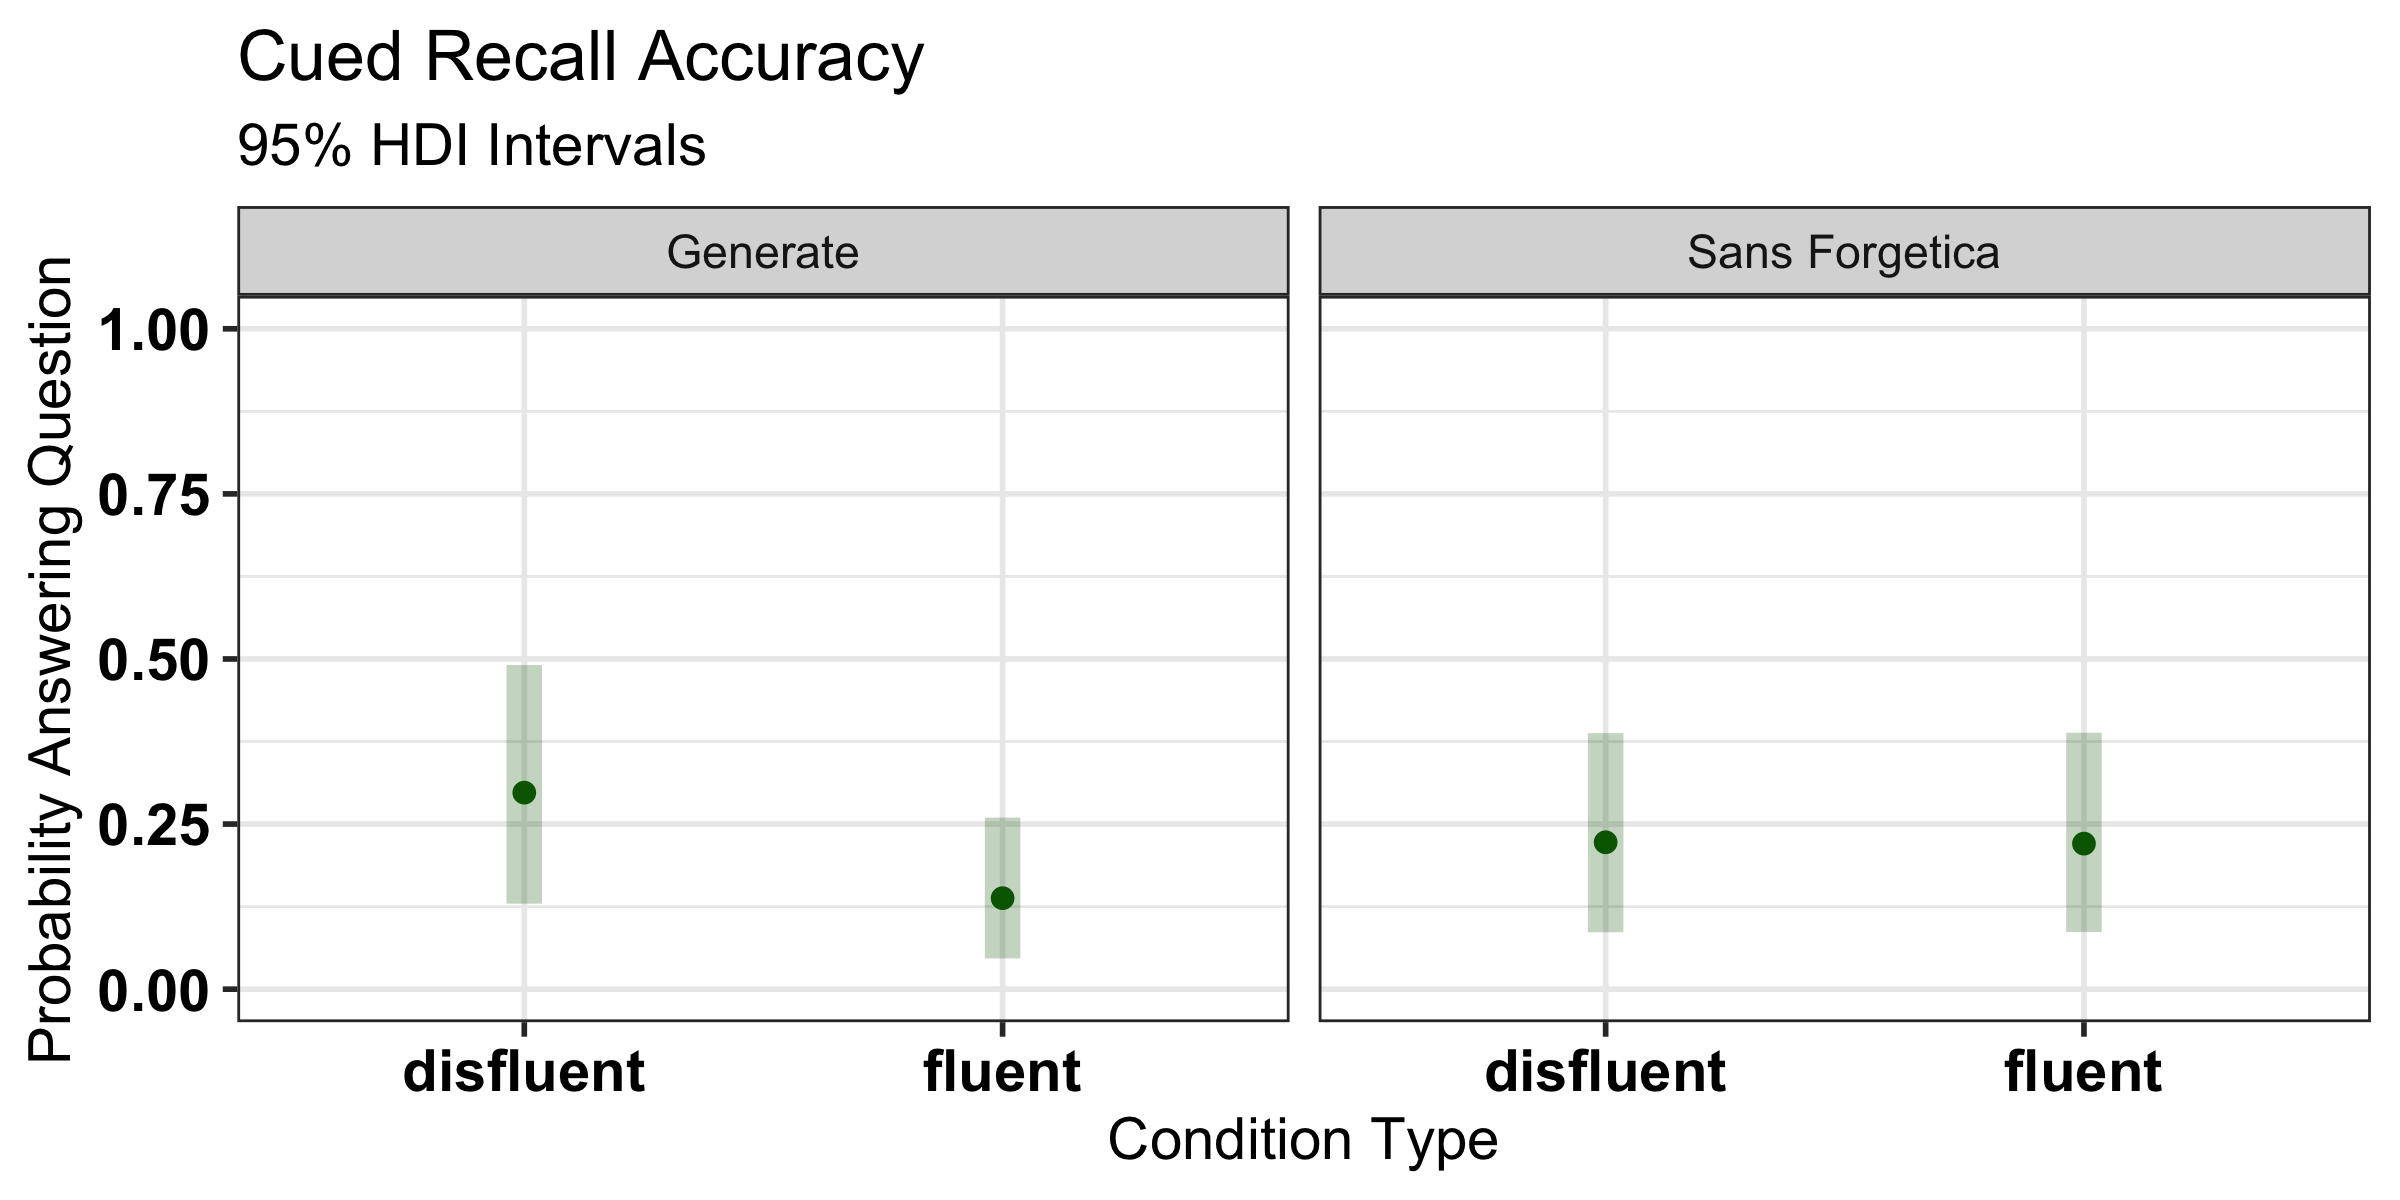
\includegraphics[width=8in]{/Users/gellr/SF_Expt2/brms_dis_plot} 

}

\caption{ }\label{fig:unnamed-chunk-2}
\end{figure}

The results for Experiment 1 are clear-cut. Cued recall performance for target pairs presented intact and in Sans Forgetica font were equivocial. That is, we did not observe a memory benefit for Sans Forgetica. We did, however, observe better cued recall performance for targets that had to be generated then when simply read, which replicates decades of litearture (cite some shit). This suggests that (1) presenting materials in Sans Forgetica does not lead to better memory and (2) the Sans Forgetica effect is most likely not generated by the same mechanisms that give rise to the generation effect.

\hypertarget{experiment-2}{%
\section{Experiment 2}\label{experiment-2}}

Experiment 1 failed to find a memory benefit for Sans Forgetica effect. One caveat of Experiment 1 is that simple paired associate learning lacks educational realsim. To remedy this, Experiment 2 tested the effects of SF using more realistic materials. Whereas Experiment 1 tested whether Sans Forgetica is driven by generation, Experiment 2 examined another possible mechanism of action--that is, the Sans Forgetcia effect might exert its mnnmenonic benefit by making material more distinctive. Specifically, Sans Forgetica may make the marked portion of text more memorable because it stands out from the surrounding text. This is similar to the effects of pre-highlighting on learning. Indeed, some evidence supports this type of role for highlighting: When students read pre-highlighted passages, they recall more of the highlighted information and less of the non-highlighted information compared to students who receive an unmarked copy of the same passage (Fowler and Barker 1974; Silvers and Kreiner 1997). To this end, Experiment 2 compared cued recall performance on a passage where some of the material were either presented in: SF, pre-highlighted in yellow, or unmarked. Each condition was manipulated between-subjects.

\hypertarget{participants-1}{%
\subsection{Participants}\label{participants-1}}

Participants were 528 undergraduates who participated for partial completion of course credit. Sample size was based on a priori power analyses conducted using PANGEA v0.2. Sample size was calculated based on the samllest effect of interest (Lakens \& Evers, 2014). Similar to Experiment 1, we were interested in powering our study to detect a medium-sized effect size (\emph{d} = .35). Therefore, assuming an alpha of .05 and a desired power of 90\%, a sample size of 170 per group is required to detect whether an effect size of .35 differs from zero. After excluding participants based on our preregistered exclusion critera, we were left with unequal group sizes. Becasue of this, we ran six more pariticpants per group, giving us 176 participants in each of the three conditions.

\hypertarget{materials-1}{%
\subsection{Materials}\label{materials-1}}

The preregistration for Experiment 2 can be found here: \url{https://aspredicted.org/3jz3z.pdf}.

Participants read a passage on ground water (856 words) taken from from the U.S. Geological Survey (see Yue et al., 2014) Eleven critical phrases\footnote{orginally we had 12 critical phrases but a pilot test showed that one of the questions was repeated twice so we removed one of them and also added a manipulation check question to sure participants were paying attention} each containing a different keyword, were selected from the passage (e.g., the term \emph{recharge} was the keyword in the phrase: Water seeping down from the land surface adds to the ground water and is called recharge water.) and were either presented in SF, highlighted, or unchanged. Then, 11 fill-in-the blank questions were created from these phrases by deleting the keyword and asking participants to provide it on the final test (e.g., Water seeping down from the land surface adds to the ground water and is called \_\_\_\_\_\_\_\_\_\_ water).

\hypertarget{design-and-procedure-1}{%
\subsection{Design and Procedure}\label{design-and-procedure-1}}

Participants were randomly assigned to either the pre-highlighted codnition, sans forgetica condition, or normal condition. Our design employed three between-subject variables: pre-highlighting, sans forgetica, and normal.

Participants completed the experiment on-line via the Qualtrics survey platform. Participant read the passage on ground water in its entirety. Participants were given 10 minutes to read the passage. Participants in the pre-highlighted condition received some of the passages in yellow highlighting. Participants in the sans forgetcia codnition were presnetd some of the sentences in the sans forgetica font. Participants in the normal passage condition were presented sentences with no changes. All particiapnts were instructed to read the passage as though they were studying material for a class.

After 10 minutes, all participants were given a brief questionnaire (2 questions) asking them to indicate their metacognitive beliefs afte reading the passage. The two questions were: \enquote{Do you feel that the presentation fo the material helped you remember} and \enquote{How likely is it that you will be able to recall material from the passage you just read on a scale of 0 (not likely to recall) to 100 (likely to recall) in 5 minutes?} Participants were then given a short distractor task (anagrams) for 3 minutes. Finally, all participants were given 11 fill-in-the-blank test questions, one at a time. There was 1 manipulation multiple choice questions: What was the passage you read on?."

\hypertarget{results-1}{%
\section{Results}\label{results-1}}

We fit a logistic mixed model in a similar fashion to Experiment 1. We fit a model with passage type as a fixed effect and random intercepts for subjects (\emph{n}=528) and questions (\emph{n}=11): (formual: acc=glmer(auto\_acc\textasciitilde{}passage\_type+(1\textbar{}Participant) + (1\textbar{}Question), data=data, family=\enquote{binomial}). Standardized parameters were obtained by fitting the model on a standardized version of the dataset. The model's total explanatory power is substantial (conditional R2 = 0.45) and the part related to the fixed effects alone (marginal R2) is of 0.00. We hypothesized that recall for pre-highlighted and sans forgetica sentences would be better remembered than normal sentences and that there would be no recall differences between the highlighted and sans forgetia sentences. Our hypotheses were partially supported (see Figure 2). Results indicated that pre-highlighted sentences were better remembered than sentences presented normally, beta = 0.38, SE = 0.17, 95\% CI {[}0.05, 0.71{]}, std. beta = 0.38, p \textless{} .05, and were marginally better remembered than sentences presented in Sans Forgetcia,\emph{Estimate} = -.317, \emph{exp(B)} = 1.37, \emph{SE} = .168, \emph{z} = -1.89, \emph{p} = .059, \emph{d} = .76. Critically, there was no difference between sentences presented normally and in sans forgetcia (beta = 0.06, SE = 0.17, 95\% CI {[}-0.26, 0.39{]}, std. beta = 0.06, p = 0.700. A Bayes factor using the brms package (Burkner, 2015) was computed and there is moderate evidence that the effects are equal (BF = 7.47).

\begin{figure}
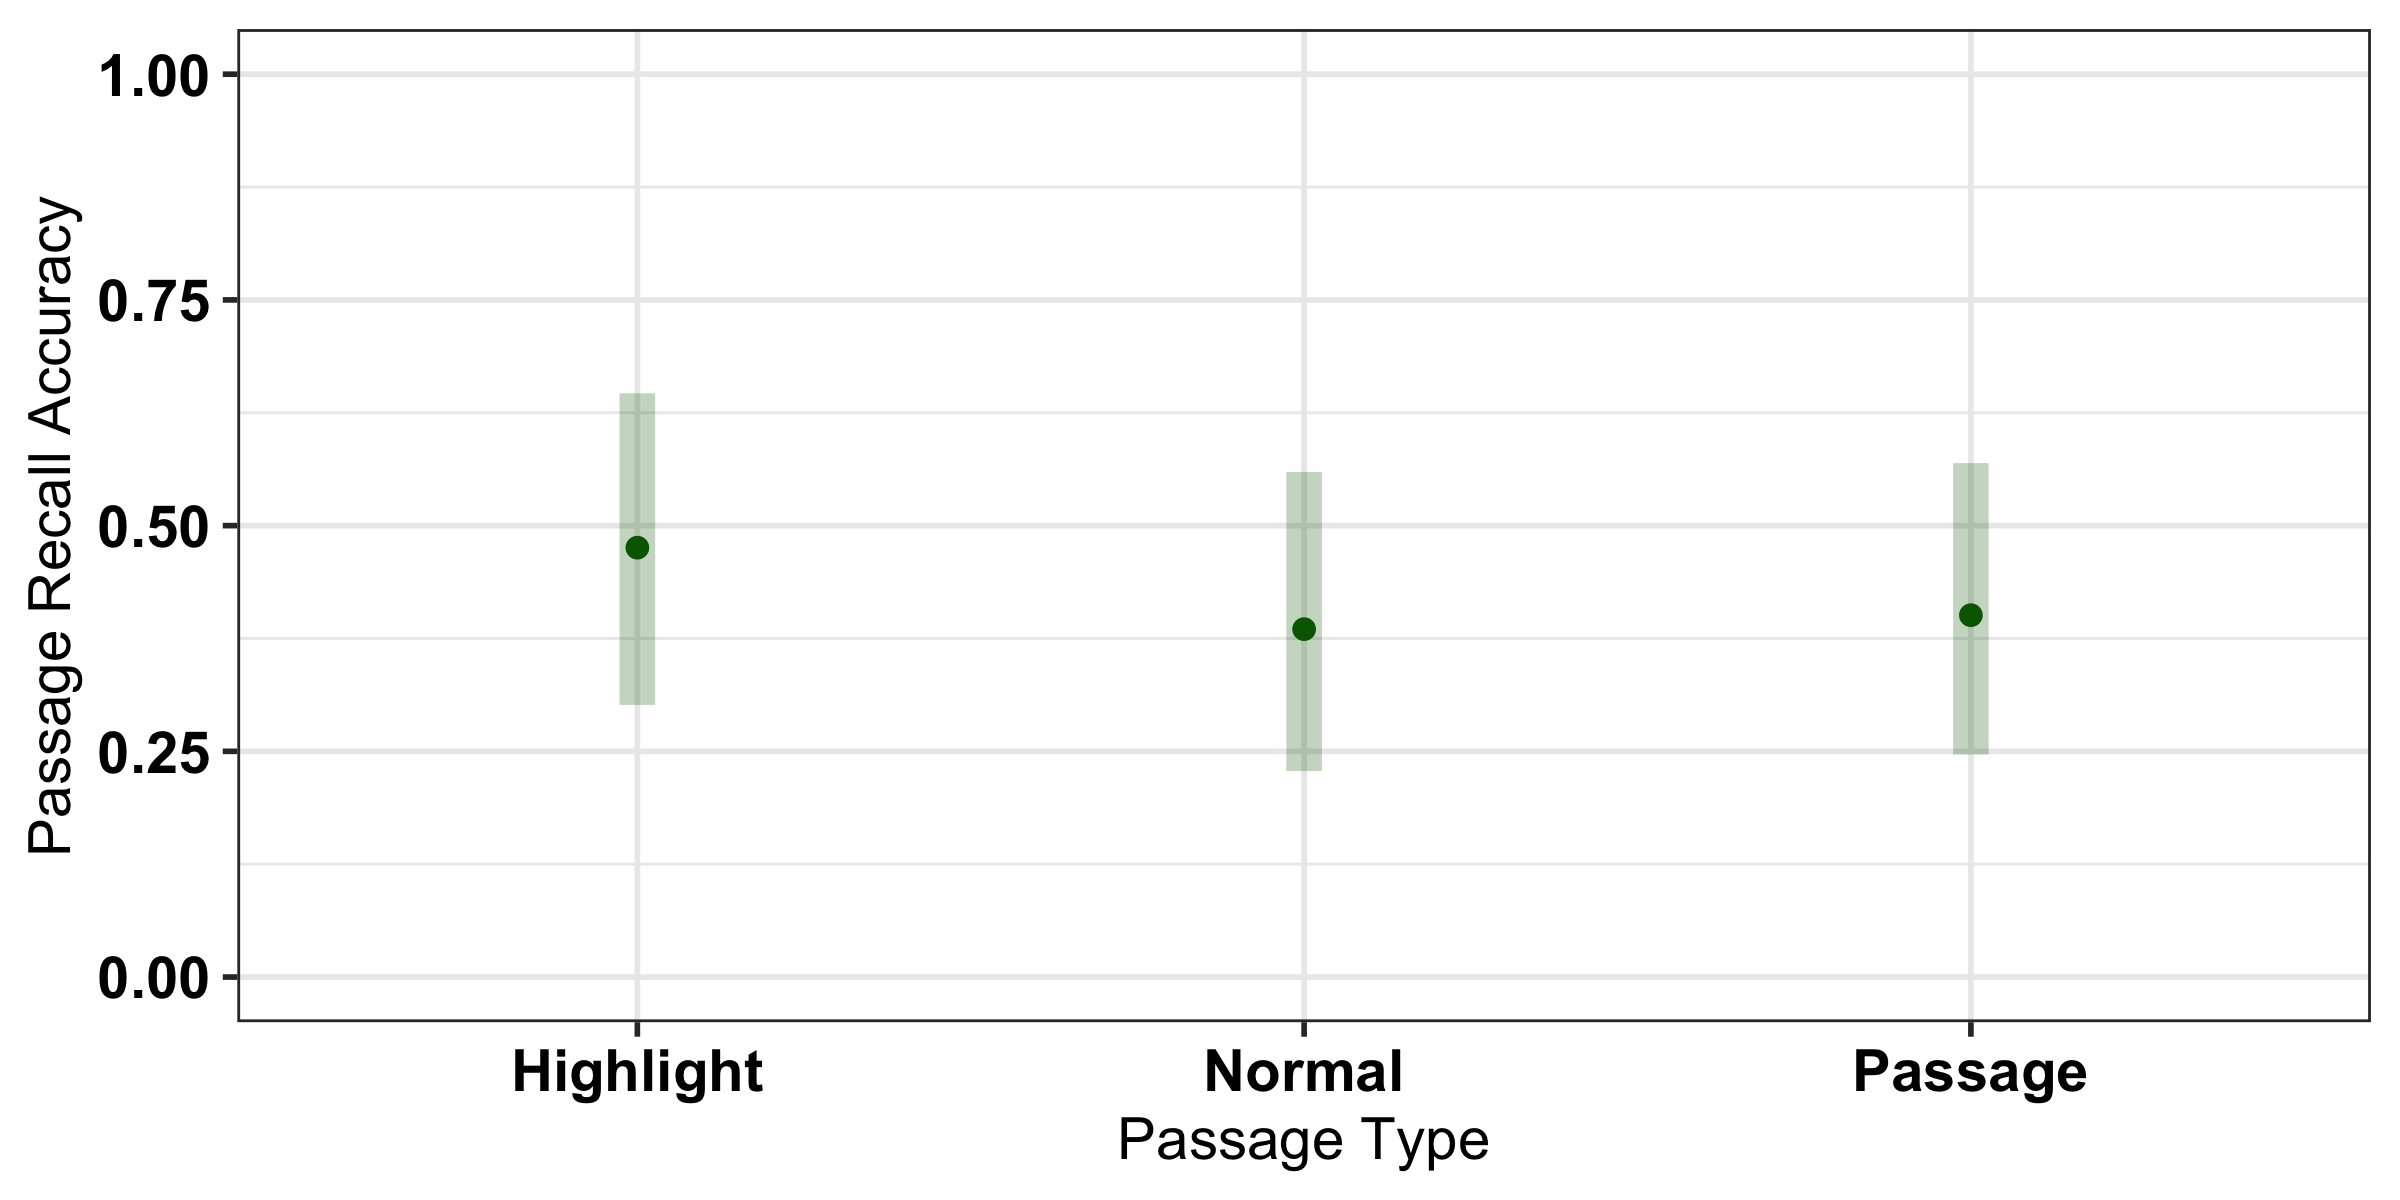
\includegraphics[width=8in]{/Users/gellr/SF_Expt2/brms_passage} \caption{ }\label{fig:unnamed-chunk-4}
\end{figure}

\hypertarget{exploratory-analysis}{%
\section{Exploratory Analysis}\label{exploratory-analysis}}

In Experiment 2 we also asked students about their metacognitive awarness. Specifically we asked participants: \enquote{How likely is it that you will be able to recall material from the passage you just read on a scale of 0 (not likely to recall) to 100 (likely to recall) in 5 minutes?} Initial analyses suggest that the normal passage was given higher JOLs (\emph{M} = 57.4, \emph{SE} = 1.97) than the pre-highlighted passage (\emph{M} = 50.3, \emph{SE} = 1.97), t(525) = -7.08, \emph{p} = .023. There were no reliable differences between the pre-highlighted passage and Sans Forgetica (\emph{M} = 53.8, \emph{SE} = 1.97), \emph{t}(525) = -3.52, \emph{p} = .415 or between the passage in Sans Forgetica and the passage presneted normally, \emph{t}(525) = 3.56, \emph{p} = .406.

One potential reason for pre-highlighted information recieving lower JOLs than the normal passage is that pre-highlighted information served to focus participants attention specific parts of the passage. Given the question, pariticpants might have thought this would hinder them if tested over the passage as a whole. Interestingly,

\begin{tabular}{l|r|r|r|r|r}
\hline
contrast & estimate & SE & df & t.ratio & p.value\\
\hline
Highlight - Normal & -7.079546 & 2.7792 & 525 & -2.547332 & 0.0299152\\
\hline
Highlight - Passage & -3.517046 & 2.7792 & 525 & -1.265488 & 0.4153929\\
\hline
Normal - Passage & 3.562500 & 2.7792 & 525 & 1.281844 & 0.4060534\\
\hline
\end{tabular}

\begin{figure}

{\centering 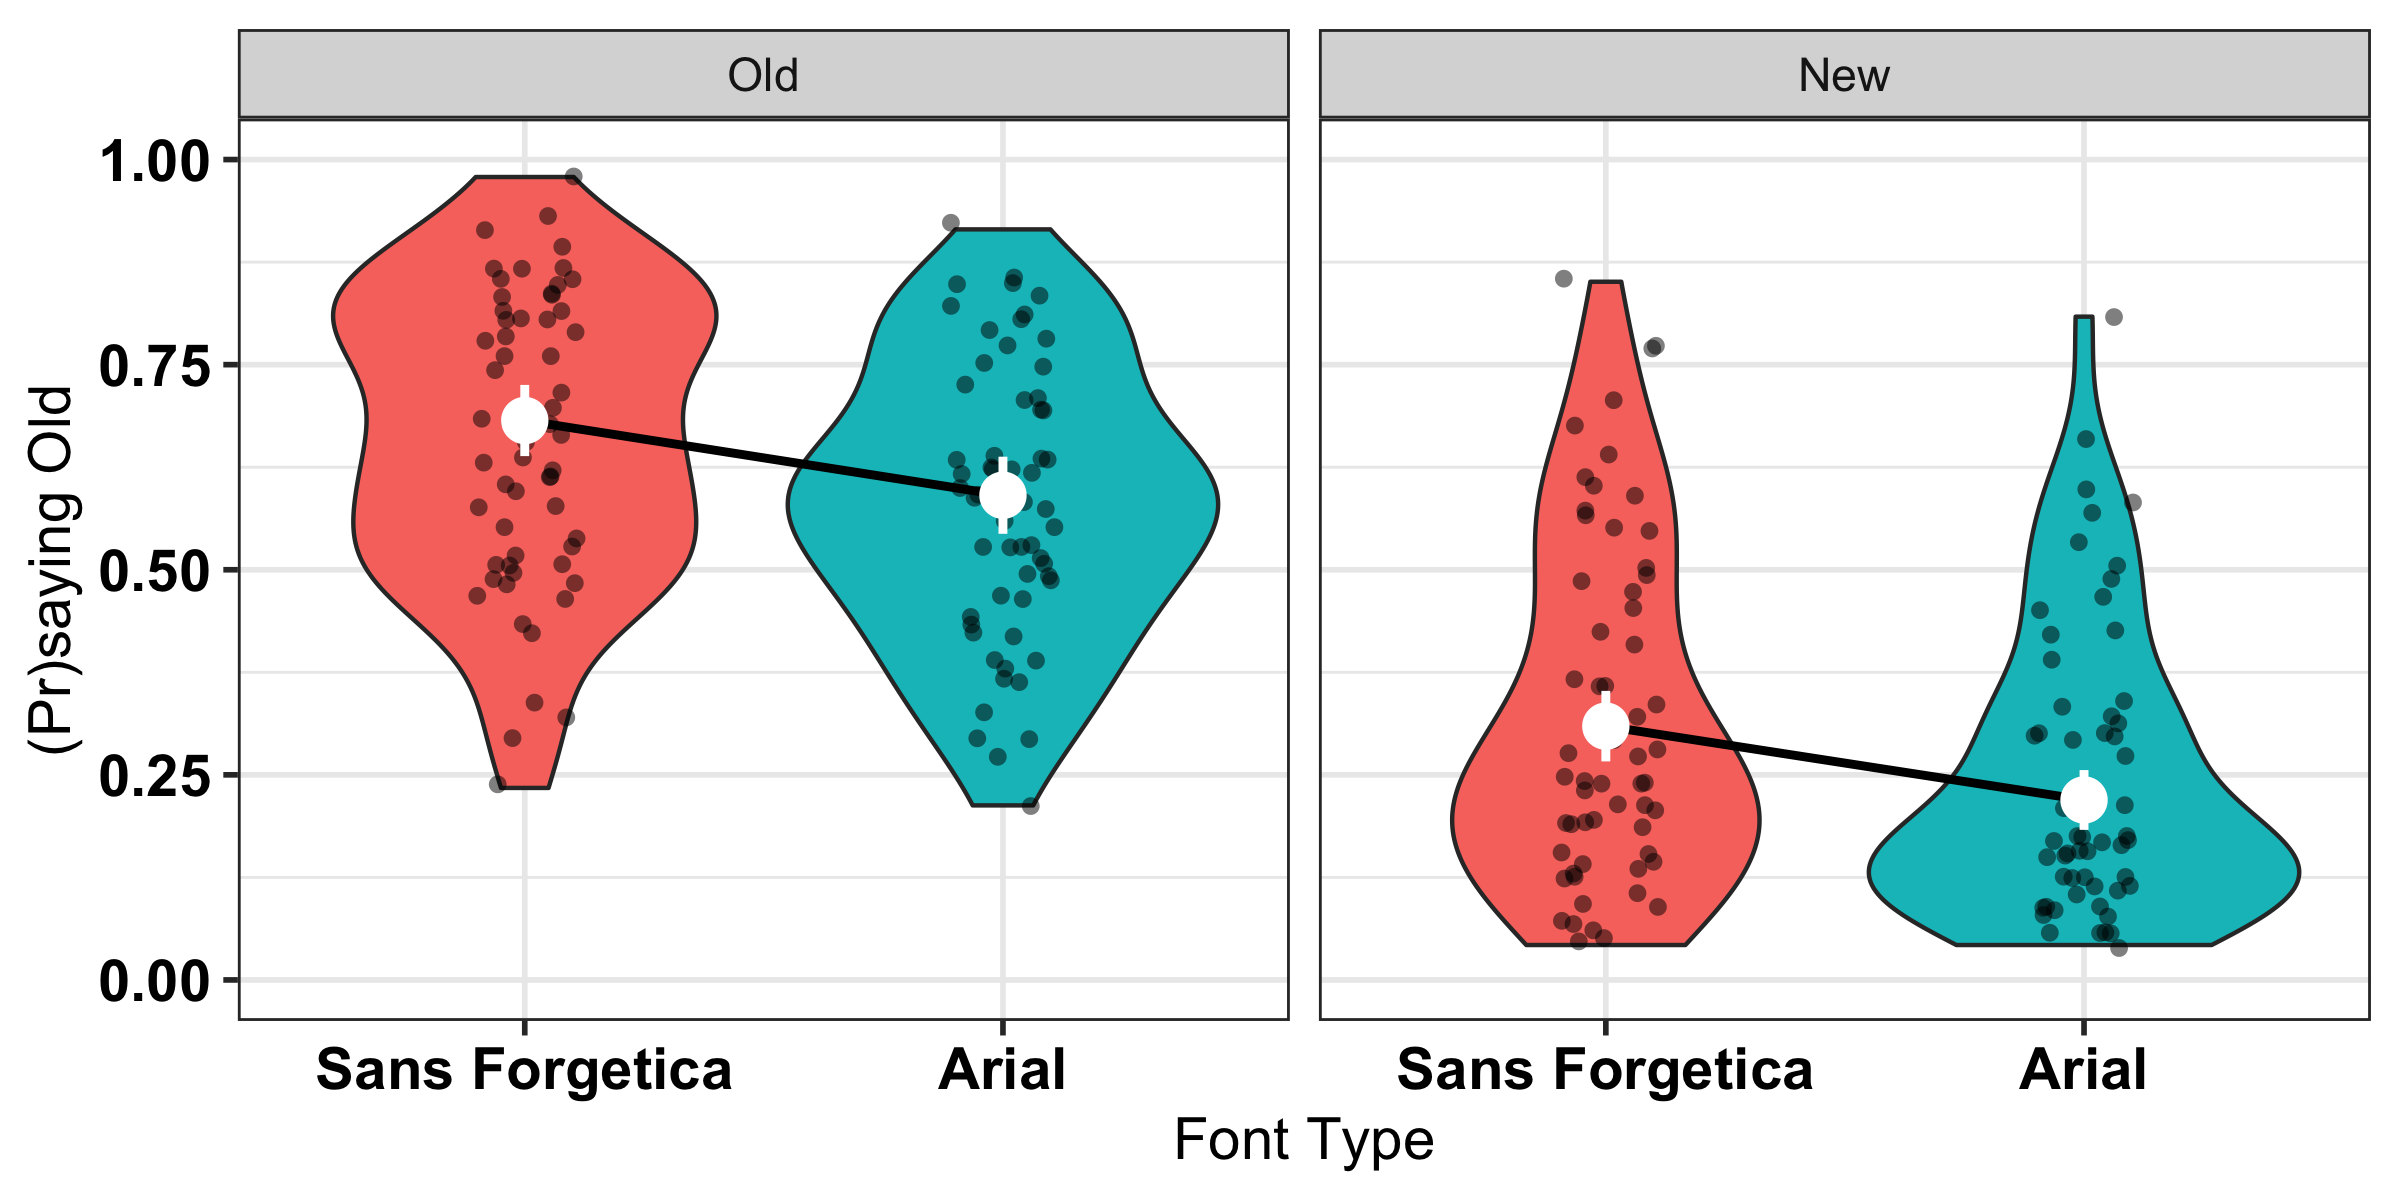
\includegraphics{SF_Paper_files/figure-latex/unnamed-chunk-5-1} 

}

\caption{Judgements of learning as a function of passage type.}\label{fig:unnamed-chunk-5}
\end{figure}

\begin{table}[tbp]
\begin{center}
\begin{threeparttable}
\caption{\label{tab:unnamed-chunk-5}}
\begin{tabular}{llllll}
\toprule
contrast & \multicolumn{1}{c}{estimate} & \multicolumn{1}{c}{SE} & \multicolumn{1}{c}{df} & \multicolumn{1}{c}{t.ratio} & \multicolumn{1}{c}{p.value}\\
\midrule
Highlight - Normal & -7.08 & 2.78 & 525.00 & -2.55 & 0.03\\
Highlight - Passage & -3.52 & 2.78 & 525.00 & -1.27 & 0.42\\
Normal - Passage & 3.56 & 2.78 & 525.00 & 1.28 & 0.41\\
\bottomrule
\end{tabular}
\end{threeparttable}
\end{center}
\end{table}

NULL

\hypertarget{dicussion}{%
\section{Dicussion}\label{dicussion}}

Across two experiment
The evidence contained herein suggests that SF does not have the mnemonic effects pruported by its creators. Now it is possible that there is an effect of SF, but the effect size might be smaller than we could detect acorss our two studies. Our SESOI was d = .35. If so, it probably does not have any real educational benefit. It is our conclsuion that SF is really forgetable and you should not be using it as a way to boost leanring.

\newpage

\hypertarget{references}{%
\section{References}\label{references}}

\begingroup
\setlength{\parindent}{-0.5in}
\setlength{\leftskip}{0.5in}

\hypertarget{refs}{}

\endgroup

\end{document}
